% Sección II: Datos hospitalarios y reconstrucción del flujo asistencial
% evidencia:E03,E06,E07,E19

\section{Datos hospitalarios y reconstrucción del flujo asistencial}

El análisis parte del repositorio PostgreSQL de solo lectura en esquema OMOP CDM v5.4~\cite{ohdsi54,mediflow2026inventario}. Conforme al principio de privacidad del certamen, ninguna etapa descarga filas individuales de pacientes ni identificadores clínicos: las extracciones se ejecutan en origen mediante 24 consultas SQL agregadas que exportan únicamente conteos por hora, día, mes o concepto hacia almacenamiento local protegido fuera de Git~\cite{mediflow2026informe,mediflow2026auditoria}.

\subsection{Esquema OMOP disponible frente a uso efectivo y cortes temporales}

Una distinción metodológica indispensable separa las tablas visibles en el catálogo OMOP del subconjunto efectivamente usado en modelos y simulaciones (Tabla~\ref{tab:omop_uso}). Aunque la base expone siete tablas principales de gran volumen, los diagnósticos, procedimientos y mediciones de laboratorio no ingresan como predictores en la matriz del modelo de demanda.

\begin{table*}[t]
\caption{Tablas OMOP inventariadas frente a uso efectivo, granularidad y restricciones observadas}
\label{tab:omop_uso}
\centering
\footnotesize
\begin{tabularx}{\textwidth}{@{}L{0.22\textwidth} r r Y@{}}
\toprule
Tabla OMOP & Filas est. & Tamaño & Uso efectivo y restricciones observadas \\
\midrule
\texttt{procedure\_occurrence} & 47,0\,M & 3,86\,GB & Solo catálogo agregado de frecuencias ($\ge 10$ registros); sin hora de procedimiento; no entra como predictor \\
\texttt{condition\_occurrence} & 38,6\,M & 3,79\,GB & Solo frecuencias agregadas de conceptos ($\ge 10$ registros); no entra en la matriz de variables de demanda \\
\texttt{measurement} & 16,6\,M & 15,0\,GB & Solo frecuencias agregadas; faltan \texttt{unit\_concept\_id} y tipo; no se integra como predictor \\
\texttt{concept} & 10,0\,M & 1,07\,GB & Diccionario de traducción de identificadores de concepto a etiquetas legibles \\
\texttt{visit\_detail} & 3,28\,M & 318\,MB & Base efectiva para etapas, duración, transiciones y censo horario; carece de \texttt{person\_id} directo (enlace vía \texttt{visit\_occurrence}) \\
\texttt{visit\_occurrence} & 1,71\,M & 153\,MB & Fuente única para llegadas diarias y horarias; inicio igual a fin en el extracto, inútil para medir estancias \\
\texttt{person} & 912\,k & 92\,MB & Solo cruce SQL para sexo y grupo etario por año de nacimiento (\texttt{13\_llegadas\_diarias\_perfil.sql}) \\
\bottomrule
\end{tabularx}
\ieeenota{Volumetría archivada del inventario del 15 de octubre de 2026 sobre estimación de catálogo PostgreSQL~\cite{mediflow2026inventario}; esquema según OMOP CDM v5.4~\cite{ohdsi54}. En el extracto faltan además \texttt{preceding\_visit\_occurrence\_id}, \texttt{visit\_type\_concept\_id} y \texttt{procedure\_datetime}.}
\end{table*}

No existe un único corte temporal compartido por todos los productos. Las series de demanda desde \texttt{visit\_occurrence} cubren del 1 de enero de 2023 sin meses vacíos al 16 de julio de 2026 como último día completo, con corte exclusivo automático en \texttt{2026-07-17} implementado en \texttt{fecha\_corte}~\cite{mediflow2026inventario,mediflow2026bundle}; registros tardíos sueltos hasta el 13 de agosto de 2026 se descartan para evitar semanas artificialmente bajas. El balance de censo en Hospitalización extiende la ventana hasta las últimas salidas el 18 de julio de 2026 a las 06:00~\cite{mediflow2026informe}, mientras el modelo Power BI PBIP opera con parámetro explícito \texttt{FechaCorte = 2026-04-30}~\cite{mediflow2026pbip}. Estas ventanas deben mantenerse diferenciadas.

\subsection{Población de visitas y etapas asistenciales}

En \texttt{visit\_occurrence}, la unidad de pronóstico es la llegada única por \texttt{visit\_concept\_id} y día (Tabla~\ref{tab:volumen_visitas}). Tres servicios concentran la demanda modelada directamente: Rehabilitación Ambulatoria (\texttt{581479}), Urgencias (\texttt{9203}) y Tratamiento Urgencias (\texttt{3045729}). Hospitalización (\texttt{9201}, 592 visitas principales, $\approx 0{,}5$/día) y 2 registros sin concepto mapeado (\texttt{0}) se agrupan en la serie residual \texttt{Otros} (código \texttt{-1}) para evitar distorsiones de métricas relativas ante días nulos~\cite{mediflow2026inventario}.

\begin{table}[htbp]
\caption{Volumen archivado por tipo de visita en \texttt{visit\_occurrence}}
\label{tab:volumen_visitas}
\centering
\scriptsize
\begin{tabularx}{\columnwidth}{@{}Y r r L{0.25\columnwidth}@{}}
\toprule
Tipo de visita (\texttt{visit\_concept\_id}) & Visitas & Prom./d & Decisión analítica \\
\midrule
Ambulatory Rehab. Visit (\texttt{581479}) & \num{1089461} & $\approx 827$ & Se modela \\
Emergency Room Visit (\texttt{9203}) & \num{598088} & $\approx 443$ & Se modela \\
Treatment urgency (\texttt{3045729}) & \num{17858} & $\approx 15$ & Se modela (diario) \\
Inpatient Visit (\texttt{9201}) & \num{592} & $\approx 0{,}5$ & Agrupada en \texttt{Otros} \\
No matching concept (\texttt{0}) & \num{2} & $\approx 0$ & Agrupada en \texttt{Otros} \\
\bottomrule
\end{tabularx}
\ieeenota{Cifras archivadas de inventario~\cite{mediflow2026inventario} previas a la agregación por corte. La baja frecuencia de Hospitalización en visitas principales no implica baja ocupación: la estancia en piso aparece masivamente como etapa en \texttt{visit\_detail}.}
\end{table}

Dado que en \texttt{visit\_occurrence} se cumple \texttt{visit\_end\_datetime} $=$ \texttt{visit\_start\_datetime} (duración mediana y $p_{90}$ iguales a 0\,h)~\cite{mediflow2026inventario}, el análisis de permanencias, ocupación y flujo se traslada íntegramente a \texttt{visit\_detail}, donde operan cuatro conceptos administrativos equivalentes (sin salas físicas, camas habilitadas ni etiquetas de \textit{triage} u observación). Allí, Hospitalización (\texttt{9201}) alcanza \num{108601} etapas válidas~\cite{mediflow2026saturacion}.

\subsection{Reconstrucción de censo horario, calentamiento y balance de stock}

Para reconstruir pacientes concurrentes por etapa en cada hora $t$ (con regularización de grilla incluyendo ceros), \texttt{serie\_censo\_etapas} aplica la ecuación de conservación discreta:
\begin{equation}
\label{eq:balance_censo}
N(t) = N_0 + E(t) - S(t),
\end{equation}
donde $N_0$ es el stock inicial en $t_0 = \text{\texttt{2023-01-01 00:00:00}}$, $E(t)$ las entradas acumuladas (\texttt{inicio < t}) y $S(t)$ las salidas acumuladas (\texttt{fin < t}), contrastadas contra el conteo directo $\text{inicio} < t \land \text{fin} \ge t$~\cite{mediflow2026informe,mediflow2026saturacion}.

Con base en el percentil 99 histórico sin recorte de Hospitalización (550,9\,h), \texttt{calcular\_calentamiento} fija un calentamiento de 24 días ($\lceil 550{,}9 / 24 \rceil + 1 = 24\text{\,d}$)~\cite{mediflow2026saturacion}. Descartar esa zona transitoria inicial evita sesgar percentiles posteriores, aunque no restauraría un $N_0$ omitido si hubiese pacientes previos a $t_0$. En~\cite{mediflow2026informe} consta una verificación archivada sobre PostgreSQL en 12 cortes horarios desde \texttt{2023-01-01 00:00} hasta \texttt{2026-07-18 06:00}: en las cuatro variantes comprobadas resultó $N_0 = 0$ y la diferencia entre $N_0 + E(t) - S(t)$ y el conteo directo fue exactamente cero en todos los cortes (Anexo~B). Dicha constatación se cita como verificación hospitalaria documentada y no fue reejecutada para este informe.

\subsection{Presión histórica por etapa y patrones descriptivos del flujo}

Sobre las series depuradas con filtro $p_{99{,}9}$ tras el calentamiento de 24 días (1.271 días observados), se definen umbrales históricos internos: verde si $\text{censo} < p_{75}$, amarillo si $p_{75} \le \text{censo} \le p_{90}$ y rojo si $\text{censo} > p_{90}$~\cite{mediflow2026saturacion} (Tabla~\ref{tab:presion_etapas}). Estos umbrales reflejan ocupación administrativa depurada, no camas físicas ni límites clínicos de seguridad.

\begin{table*}[t]
\caption{Presión histórica del censo horario por etapa tras calentamiento de 24 días y filtro $p_{99{,}9}$}
\label{tab:presion_etapas}
\centering
\footnotesize
\begin{tabularx}{\textwidth}{@{}Y r r r r r r@{}}
\toprule
Etapa (\texttt{visit\_detail}) & Mediana & $p_{75}$ & $p_{90}$ & Máx. & H/día rojo & Días en rojo \\
\midrule
Inpatient Visit (\texttt{9201}) & 283,0 & 297,0 & 309,0 & 359,0 & 2,2 & 19,2\,\% \\
Treatment urgency (\texttt{3045729}) & 201,0 & 239,0 & 272,0 & 518,0 & 2,4 & 37,9\,\% \\
Emergency Room Visit (\texttt{9203}) & 0,0 & 1,0 & 3,0 & 162,0 & 1,0 & 57,0\,\% \\
Ambulatory Rehab. (\texttt{581479}) & 0,0 & 0,0 & 0,0 & 0,0 & 0,0 & 0,0\,\% \\
\bottomrule
\end{tabularx}
\ieeenota{Datos archivados de~\cite{mediflow2026saturacion} (secs. 3--4, 19 de noviembre de 2026, 1.271 días poscalentamiento) excluyendo duraciones $>p_{99{,}9}$. En Rehabilitación Ambulatoria la duración registrada es 0,0\,h (censo nulo y 24\,h en amarillo al coincidir $p_{75}=p_{90}=0$). En Urgencias (\texttt{9203}), $p_{90}=3$ hace roja cualquier hora con $\ge 4$ registros simultáneos.}
\end{table*}

Las Figs.~\ref{fig:exploracion_llegadas}--\ref{fig:exploracion_duracion} muestran la concentración matutina de llegadas (pico en Urgencias de 08:00 a 14:00; actividad laboral en Rehabilitación con caídas en fines de semana y festivos), la tendencia 2023--2026 con valles en Carnaval, Semana Santa y fin de año, y el alargamiento vespertino/nocturno de Tratamiento Urgencias~\cite{mediflow2026informe}. Se excluye la figura exploratoria histórica \texttt{04\_censo\_etapas.png}, generada antes del filtro $p_{99{,}9}$ (exhibe medianas de Urgencias de 6--7 y $p_{90}$ de Hospitalización $>320$, incompatibles con la Tabla~\ref{tab:presion_etapas}).

\begin{figure*}[t]
\centering
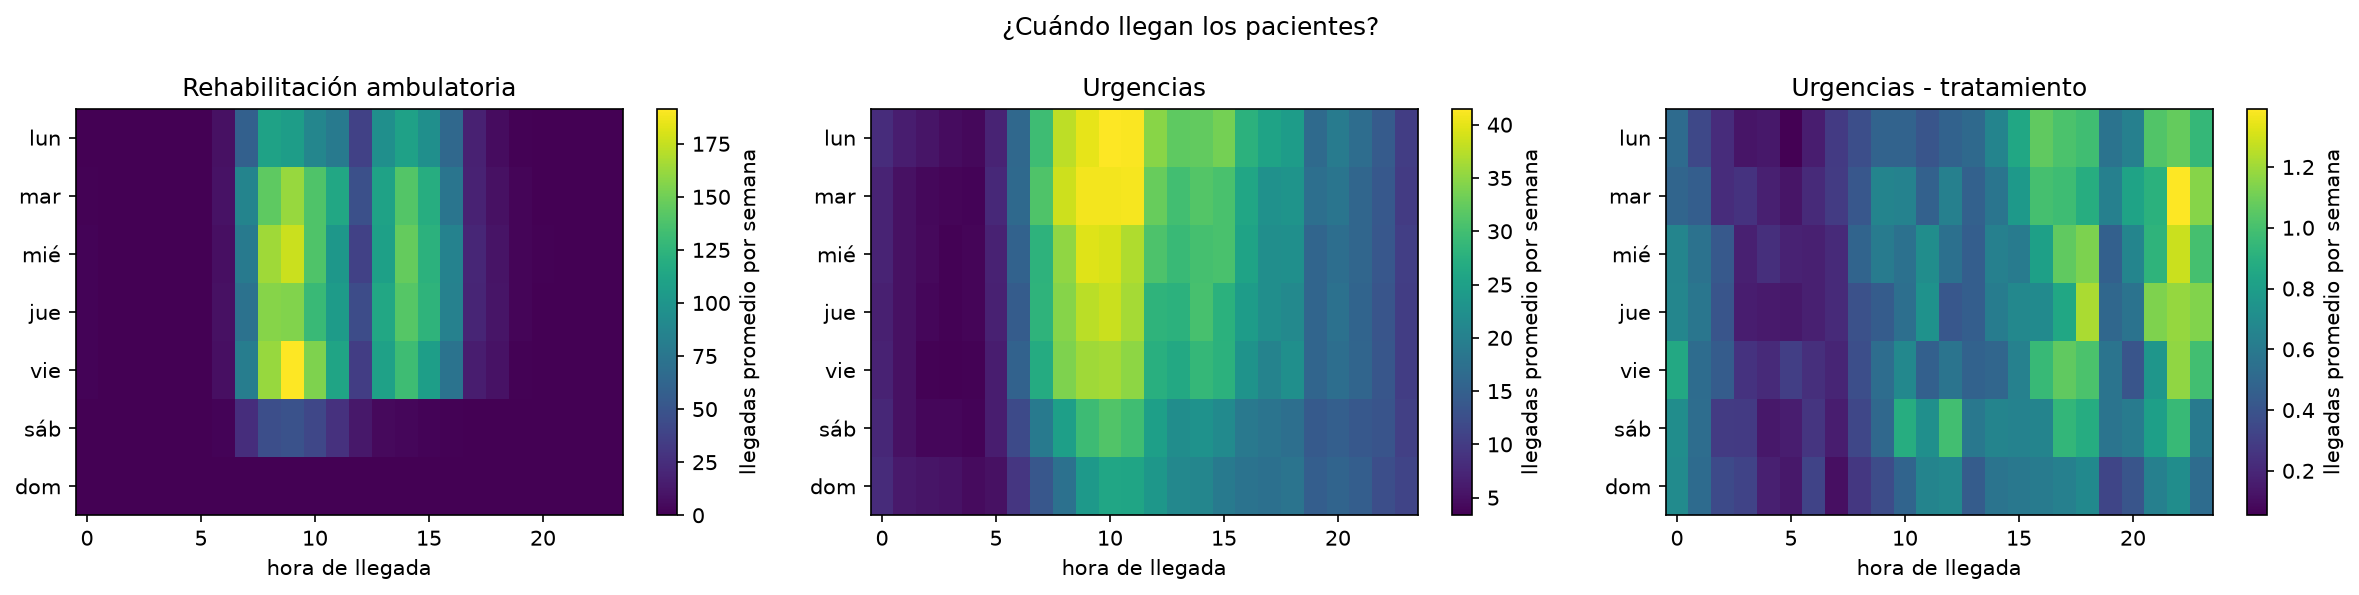
\includegraphics[width=0.96\textwidth]{01_llegadas_dia_hora.png}
\caption{Patrones descriptivos de llegadas promedio por hora y día de la semana (\protect\nolinkurl{01_llegadas_dia_hora.png}). Refleja distribución histórica archivada y no rendimiento predictivo.}
\label{fig:exploracion_llegadas}
\vspace{4pt}
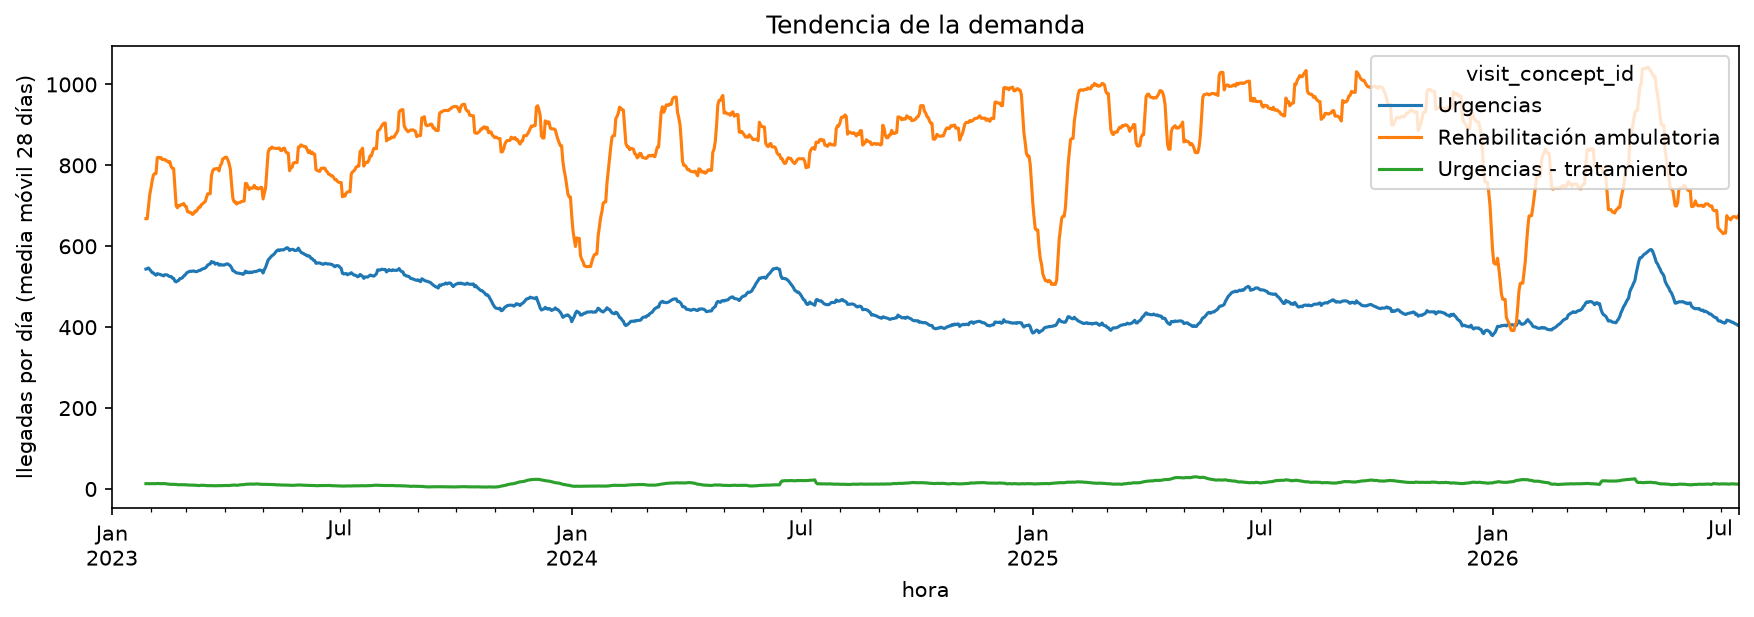
\includegraphics[width=0.96\textwidth]{02_tendencia.png}
\caption{Tendencia histórica de llegadas diarias en media móvil de 28 días, 2023--2026 (\protect\nolinkurl{02_tendencia.png}). Muestra descensos estacionales de Rehabilitación sin proyecciones fuera de muestra.}
\label{fig:exploracion_tendencia}
\vspace{4pt}
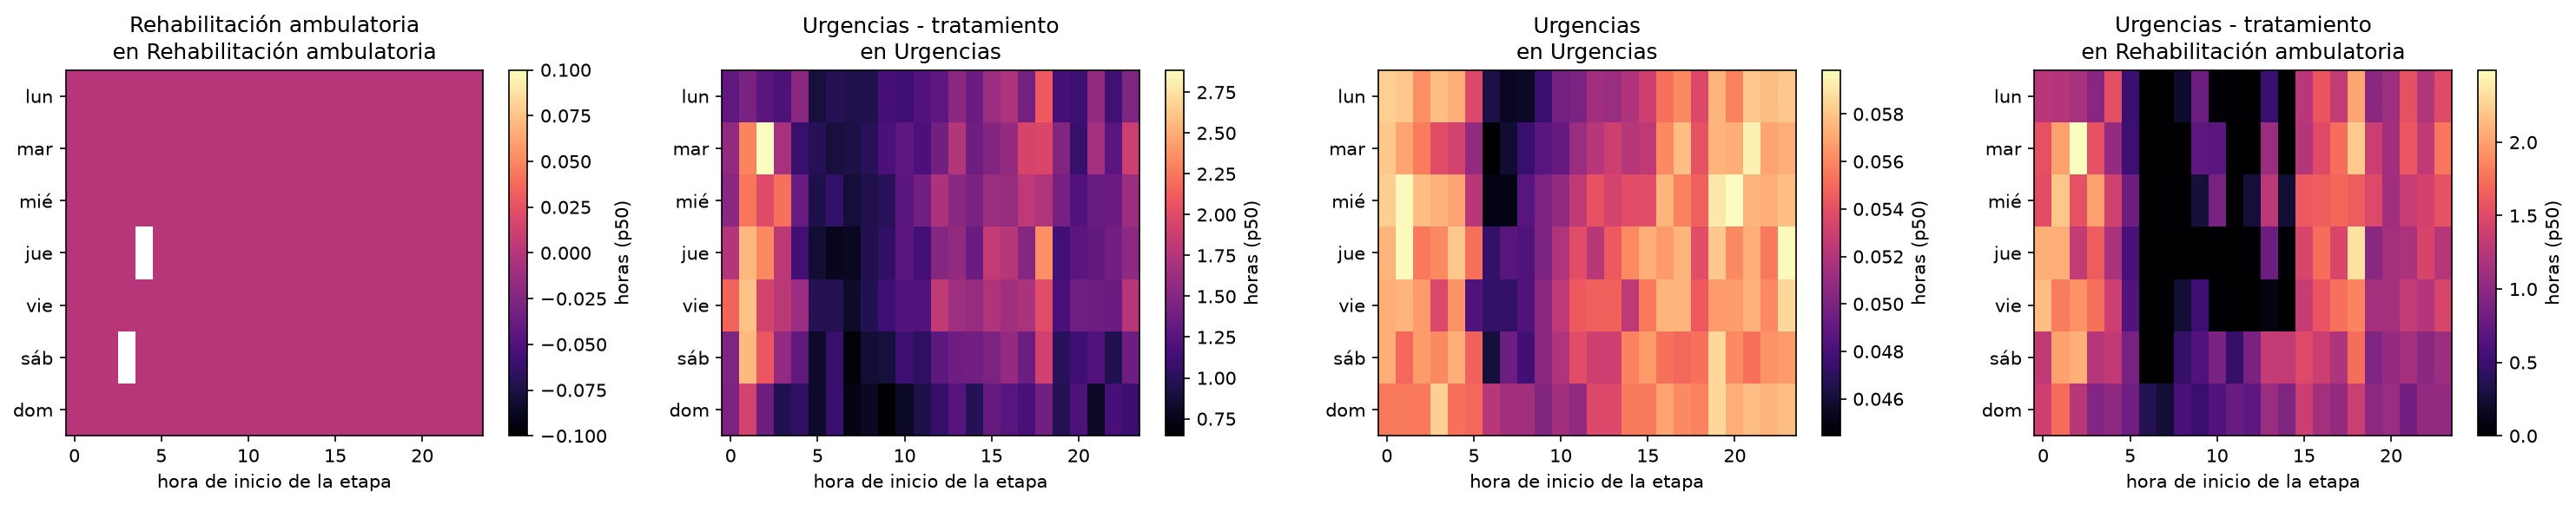
\includegraphics[width=0.96\textwidth]{03_duracion_etapas_franja.png}
\caption{Duración mediana (percentil 50) de etapas según día y hora de inicio (\protect\nolinkurl{03_duracion_etapas_franja.png}). Los valores nulos en Rehabilitación obedecen a ausencia de marcas de salida distintas del inicio.}
\label{fig:exploracion_duracion}
\end{figure*}

\subsection{Transición prioritaria entre Tratamiento Urgencias y Hospitalización}

La consulta \texttt{18\_transiciones\_etapas.sql} identifica como transición prioritaria el salto desde \textit{Treatment urgency} (\texttt{3045729}) hacia \textit{Inpatient Visit} (\texttt{9201}) dentro de visitas de Urgencias (\texttt{9203}), con \textbf{\num{47670} pasos}~\cite{mediflow2026optimizacion}. Con $\text{espera\_h} = \text{inicio\_siguiente} - \text{fin\_anterior}$, el $p_{50}$ mensual ponderado es \num{0,0}\,h y el $p_{90}$ mensual ponderado alcanza \textbf{\num{24,45}\,h} (\num{24,446}\,h sin redondear). Tres advertencias limitan su lectura: (1) admite valores negativos por solapamiento administrativo y no equivale a espera clínica por cama ni mide \textit{boarding}; (2) \num{24,45}\,h es el promedio mensual ponderado de $p_{90}$ y no el $p_{90}$ global de los \num{47670} registros agrupados; y (3) al cruzar mensualmente ese $p_{90}$ con el censo medio de Hospitalización surge una correlación ecológica negativa ($r = -0{,}481$; $p_{90}$ ponderado de \num{25,13}\,h en meses normales frente a \num{23,70}\,h en meses de censo alto)~\cite{mediflow2026optimizacion}, descartando una atribución causal simple a la congestión de piso sin auditar marcas en el HIS.
